% --
% onset

\section{Onset Detection}\label{sec:signal_onset}
\thesisStateReady
\thesisStateNew
Onset detection of key words is an essential part in Key Word Spotting (KWS) systems and describes the starting time of an actual key word.
In this thesis the onset detection is separated into:
\begin{itemize}
  \item key word onset detection (within a fixed time span)
  \item online onset detection
\end{itemize}
the key word onset detection is performed on already extracted time signals, such as raw data examples from the dataset, where the time interval of those signals are limited to \SI{1}{\second}.
The online onset detection runs during the recording of potential key words from a microphone input in a real time system.
Note that onset detection can be quite challenging and is of some sorts an own research subject.
For this thesis, however it is enough to use trivial methods, that do not use much computational effort.


% --
% key word onset detection

\subsection{Key Word Onset Detection}\label{sec:signal_onset_kw}
An intuitive method to detect the onsets of key words in a fixed time signal, is to simply use the signal energy.
Consider a fixed time signal $\bm{x} \in \R^n$ with a total number of $n$ samples, that is windowed with a striding frame of sample length $N$ corresponding to a time duration of \SI{500}{\milli\second}, the energy of each windowed signal is calculated as:
\begin{equation}\label{eq:e_win}
  e[m] = \sum_{i=0}^{N-1} \abs{x[m + i]}^2
\end{equation}
with shift index $m \in \mathcal{M} = \{0, 1, \dots, n - N + 1\}$.
The onset sample number $o \in \mathcal{M}$ with the highest energy region can be determined by
\begin{equation}\label{eq:onset}
  o = \underset{m \in \mathcal{M}}{\arg \max} \, e[m]
\end{equation}
for all windowed signal energies $e[m]$.
Note that it is assumed, that most of the key word in each signal is captured by the window length $N$ and that no noise peaks are present before and after the key word, otherwise the onset $o$ is shifted to either the left or right-hand side of the actual key word onset.
It is for sure, that this onset detection is not the most reliable one, but it is the simplest and most energy efficient method performed on raw audio data.

A better approach is to use energy values from the frequency response of the signal.
Since the Mel Frequency Cepstral Coefficients (MFCC) are extracted to obtain features for neural networks, it is straight forward to use them for onset detection as well.
The first cepstral coefficient $\bm{u}_0 \in \R^M$ of the MFCCs is actually an energy value, that is the sum of all equidistant mel filter bands.
The equivalent of \req{e_win} for MFCCs in the cepstral and frame space is therefore:
\begin{equation}
  e[m] = \sum_{i=0}^{N-1} \bm{u}_0[m + i]
\end{equation}
where $m$ and $N$ are in the frame space instead of the sample space.
A conversion from sample to frame space can simply be done by dividing the sample variable with the hop size $h$ in samples and rounding it to an integer number.
The onset frame $o$, using the first MFCC coefficient, is determined in the same way as formulated in \req{onset}.
An illustration of the onset detection with the fixed window of size \SI{500}{\milli\second} is shown in \rfig{signal_onset_window}, where
the start of the striding window with the highest energy value contained in this window, is the onset.
\begin{figure}[!ht]
  \centering
    
\includegraphics[width=0.55\textwidth]{./3_signal/figs/signal_onset_window}
  \caption{Striding window length of \SI{500}{\milli\second} used for energy calculation in onset detection.}
  \label{fig:signal_onset_window}
\end{figure}
\FloatBarrier
\noindent
A showcase on the performance of both energy onset detection methods are shown in \rfig{signal_onset_showcase}.
\begin{figure}[!ht]
  \centering
    \subfigure[left]{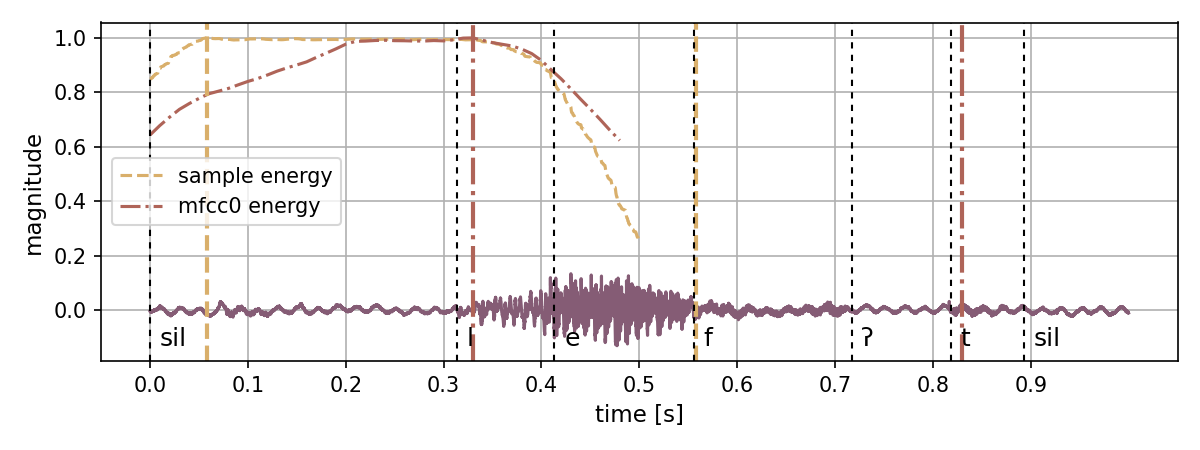
\includegraphics[width=0.45\textwidth]{./3_signal/figs/signal_onset_showcase_left0}}
    \subfigure[right]{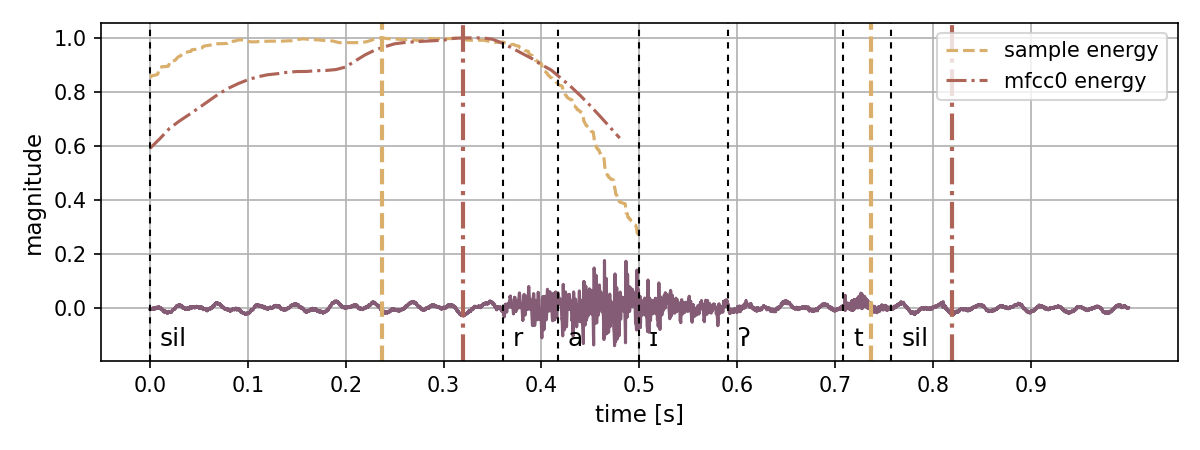
\includegraphics[width=0.45\textwidth]{./3_signal/figs/signal_onset_showcase_right0}}
    \subfigure[up]{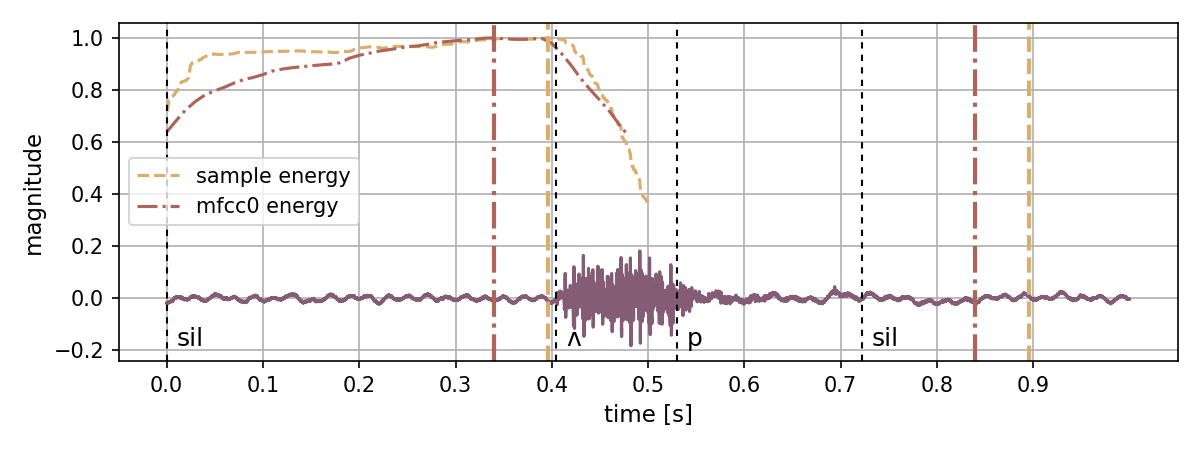
\includegraphics[width=0.45\textwidth]{./3_signal/figs/signal_onset_showcase_up0}}
    \subfigure[down]{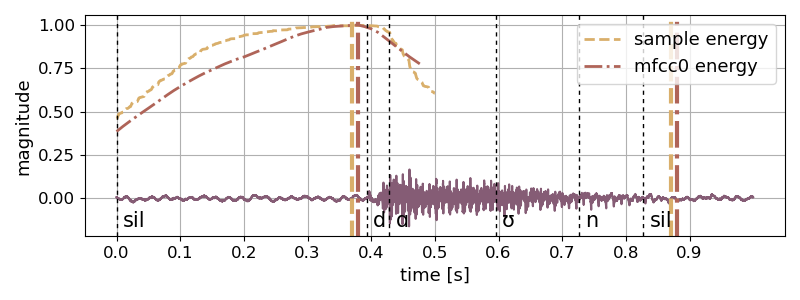
\includegraphics[width=0.45\textwidth]{./3_signal/figs/signal_onset_showcase_down0}}
    \subfigure[go]{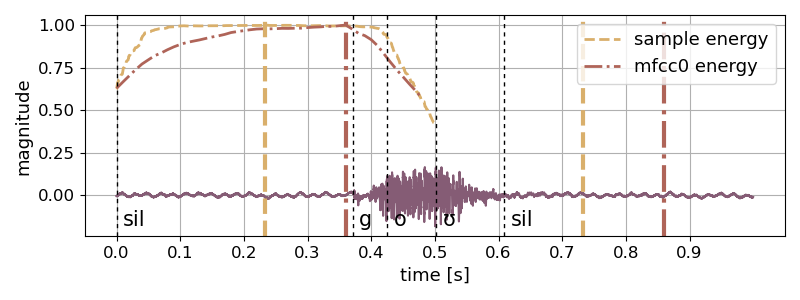
\includegraphics[width=0.45\textwidth]{./3_signal/figs/signal_onset_showcase_go0}}
  \caption{Onsets (vertical colored lines) obtained from the maximum of either the sample energy or first MFCC coefficient energy, with an analytical window length of \SI{500}{\milli\second}.}
  \label{fig:signal_onset_showcase}
\end{figure}
\FloatBarrier
\noindent
It can be observed that the MFCC onset method works much better, especially for the \enquote{left} example, where a little noise peak shifts the sample energy onset too far to the left so that the whole word is not captured.
For all MFCC extractions from the datasets during the experiments, the MFCC onset method is used. 
For raw audio extraction, applied in Wavenets, the sample energy method is applied.


% --
% key word onset detection

\subsection{Online Onset Detection}
The onset detection of online speech signals received from a microphone input stream, is processed by evaluating consecutive input chunks, that are stored in an input buffer.
From those input chunks the energy level can be computed and compared with an energy threshold, that should indicate the presence of an onset.
It is not the purpose to detect key word onsets by its correct starting time, but to signalize that a signal with enough energy is available for a potential key word classification.
Mathematically the onset $o(\bm{x}) \in \{0, 1\}$ of an input chunk $\bm{x} \in \R^n$ from an actual microphone input stream, can be obtained by:
\begin{equation}
  o(\bm{x}) = 
  \begin{cases}
    1, & \text{if } \frac{1}{n} \bm{x}^T \bm{x} > \alpha\\
    0, & \text{otherwise} 
  \end{cases}
\end{equation}
where the output value of $1$ represents the occurance of an onset, $n$ is the total sample number of the input chunk and $\alpha$ the energy threshold.
The energy threshold should be adjustable to the users microphone and ampliefier setup. 
This can be done for instance in the video game option menu as described in \rsec{game_interactables_menu}.
If an online onset is detected, the whole buffer is filled up first, then read and MFCC features extracted.
From those MFCCs the exact key word onset is calculated as described in \rsec{signal_onset_kw} and the \SI{500}{\milli\second} long feature vectors are sent to the classification system.